\chapter{Descrizione}
Le modifiche a cui si è dovuti andare incontro sulla base di dati, guidati dalle logiche per l'implementazione delle nuove funzionalità di RepominerEvo, sono state riassunte nella tabella \ref{table:description} riportata di seguito.

\begin{table}[ht]
    \begin{tabular}{|p{3cm}|p{3cm}|p{3cm}|p{3cm}|}
        \hline
        \rowcolor[gray]{.80}

        Entità & Changes(Y/N) & Descrizione del cambiamento & Impatto (Minor/Major/Nil) \\ \hline
        Schema `metrics` & Y & Aggiunte due relazioni con due nuove tabelle & Minor \\ \hline
       
 Schema relazionale & Y & Creazione di due nuove tabelle: `package\_metrics` e `project\_metrics` & Minor \\ \hline
		
        \hline
    \end{tabular}
\caption{Cambiamenti hardware e software}\label{table:description}
\end{table}

Analizzando i cambiamenti effettuati, è doveroso riportare come l'implementazione di nuove metriche di package e di progetto ci abbia spinto alla creazione di due nuovi schema per lo storage degli stessi:
\begin{itemize}
\item `package\_metrics`
\item `project\_metrics`
\end{itemize}

In figura \ref{fig:dettaglioF} di pagine \pageref{fig:dettaglioF} mostriamo le tabelle aggiunte con le relazioni create.
\medskip
\begin{figure}[ht]
	\centering
	%width=.5\textwidth
	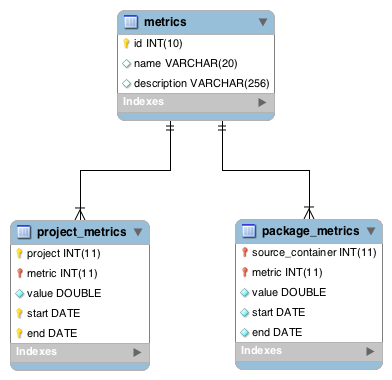
\includegraphics[width=.5\textwidth]{img/dettaglioFinal.png}
	\caption{Nuove relazioni instaurate}\label{fig:dettaglioF}
\end{figure}

Nella fase a priori di impact analysis, gli schemi di \textit{`project\_metrics`} e \textit{`package\_metrics`} erano stati ideati senza i campi per le rispettive start date ed end date. Durante lo sviluppo, si è resa necessaria questa aggiunta avendo incontrato la necessità di prevedere per una stessa metrica valori diversi su archi temporali differenti.\\

C'è da evidenziare come questi cambiamenti, mirati ad adattare la struttura della base di dati alle logiche delle nuove metriche, si siano solamente limitati all'estensione della stuttura relazionale esistente, senza tuttavia richiedere modifiche al comportamento del sistema già sviluppato, il quale potrà continuare a esercitare anche sul database così adattato senza alcuna necessità di intervento supplementare. 

Riportiamo nella figura \ref{fig:repominer} di pagina \pageref{fig:repominer} la struttura del database a seguito delle modifiche effettuatevi, per quanto riguarda le relazioni principali di interesse per il sistema implementato

\begin{figure}[t]
	\centering
	%width=.5\textwidth
	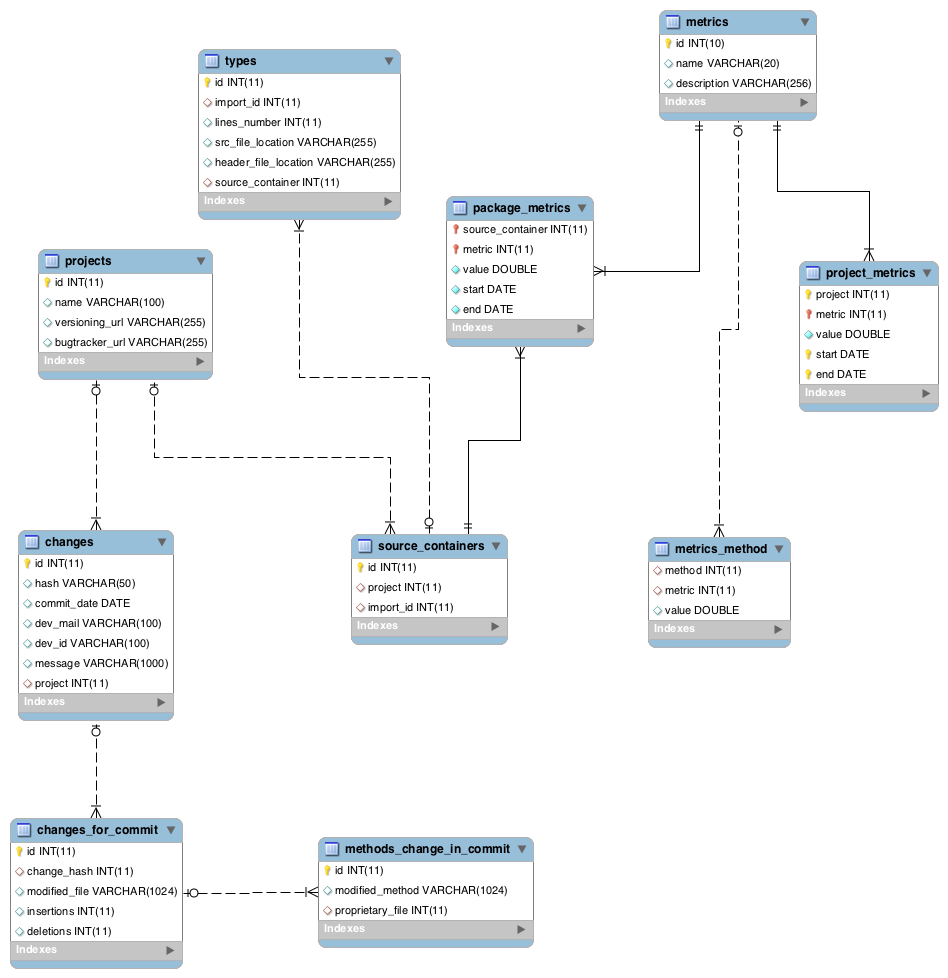
\includegraphics[width=\textwidth]{img/repominer.png}
	\caption{Dettaglio dello schema relazionale modificato}\label{fig:repominer}
\end{figure}